\chapter{Resultados \label{chap:Resultados}}
%%%%%%%%%%%%%%%%%%%%%%%%%%%%%%%%%%%%%%%%%%%%%%%%%%%%%%%%%%%%%%%%%%
%%%%%%%%%%%%%%%%%%%%%%%%%%%%%%%%%%%%%%%%%%%%%%%%%%%%%%%%%%%%%%%%%%
\section{Ajuste de espectros}
\noindent Habiendo calculado y aplicado los valores de expectación, $\mu_{g}$ y $\mu_{bkg}$, para corregir la carga sobre los clusters y habiendo introducido el modelo de la colección parcial de carga, usado en los ajustes de los espectros, ya se pueden obtener los resultados derivados de las correcciones.

Los resultados que se presentan a continuación son tanto para el pico del flúor como los picos del aluminio. Para ambos casos se muestran los histogramas de carga con sus respectivos ajustes, utilizando el modelo descripto en la Capítulo \ref{chap:ModeloPCC}, para el caso en el que se aplicó el umbral \verb|EPIX=1.5| con las correcciones. Se presentan en tablas los resultados tanto para el primer cuadrante del sensor como para el tercer cuadrante, debido a que el segundo cuadrante no funciona correctamente y el cuarto cuadrante presenta muchas \textit{hot columns}

%%%%%%%%%%%%%%%%%%%%%%%%%%%%%%%%%%%%%%%%%%%%%%%%%%%%%%%%%%%%%%%%%%
%%%%%%%%%%%%%%%%%%%%%%%%%%%%%%%%%%%%%%%%%%%%%%%%%%%%%%%%%%%%%%%%%%
\subsection{Aluminio}
\noindent Utilizando el modelo descripto en la sección \ref{chap:ModeloPCC} y el método de la máxima verosimilitud, se hizo un barrido en el parámetro $\beta$, de donde se obtuvieron las curvas del logaritmo de la verosimilitud para los cuadrantes uno y tres del sensor, las cuales se encuentran en los gráficos de la Figura \ref{fig:Al_barridos_beta}. De estas, se obtiene el máximo $\hat{\beta}$, el intervalo que lo contiene y los valores de $F$ y $\varepsilon_{\eh}$ óptimos del ajuste de los histogramas. En ambos casos se grafica la recta que se encuentra a una distancia $a=1/2$ por debajo del máximo y su intersección con la curva obtenida del barrido en $\beta$ para la verosimilitud, de donde se obtuvieron los intervalos $[0.00396, 0.01144]$ y $[0.014152, 0.023138]$ para un $68.3\,\%$ de probabilidad de contener a $\beta$, para el primer y tercer cuadrante del sensor respectivamente. 

El tamaño de la región de PCC, junto con su error se desprenden de los valores hallados para $\beta$ y de la distancia de atenuación del aluminio para los rayos $X$ de $1500\,\si{eV}$, que en este caso vale $\tau_{\scaleto{X}{4pt}} = 8.087\,\si{\mu m}$\cite{AttenuationLength}. Utilizando que $\tau_{\scaleto{CCE}{4pt}} = \beta \tau_{\scaleto{X}{4pt}}$ se obtiene que $\tau_{\scaleto{CCE}{4pt}} = algo \pm otra cosa$.

\begin{figure}[h]
    \centering
        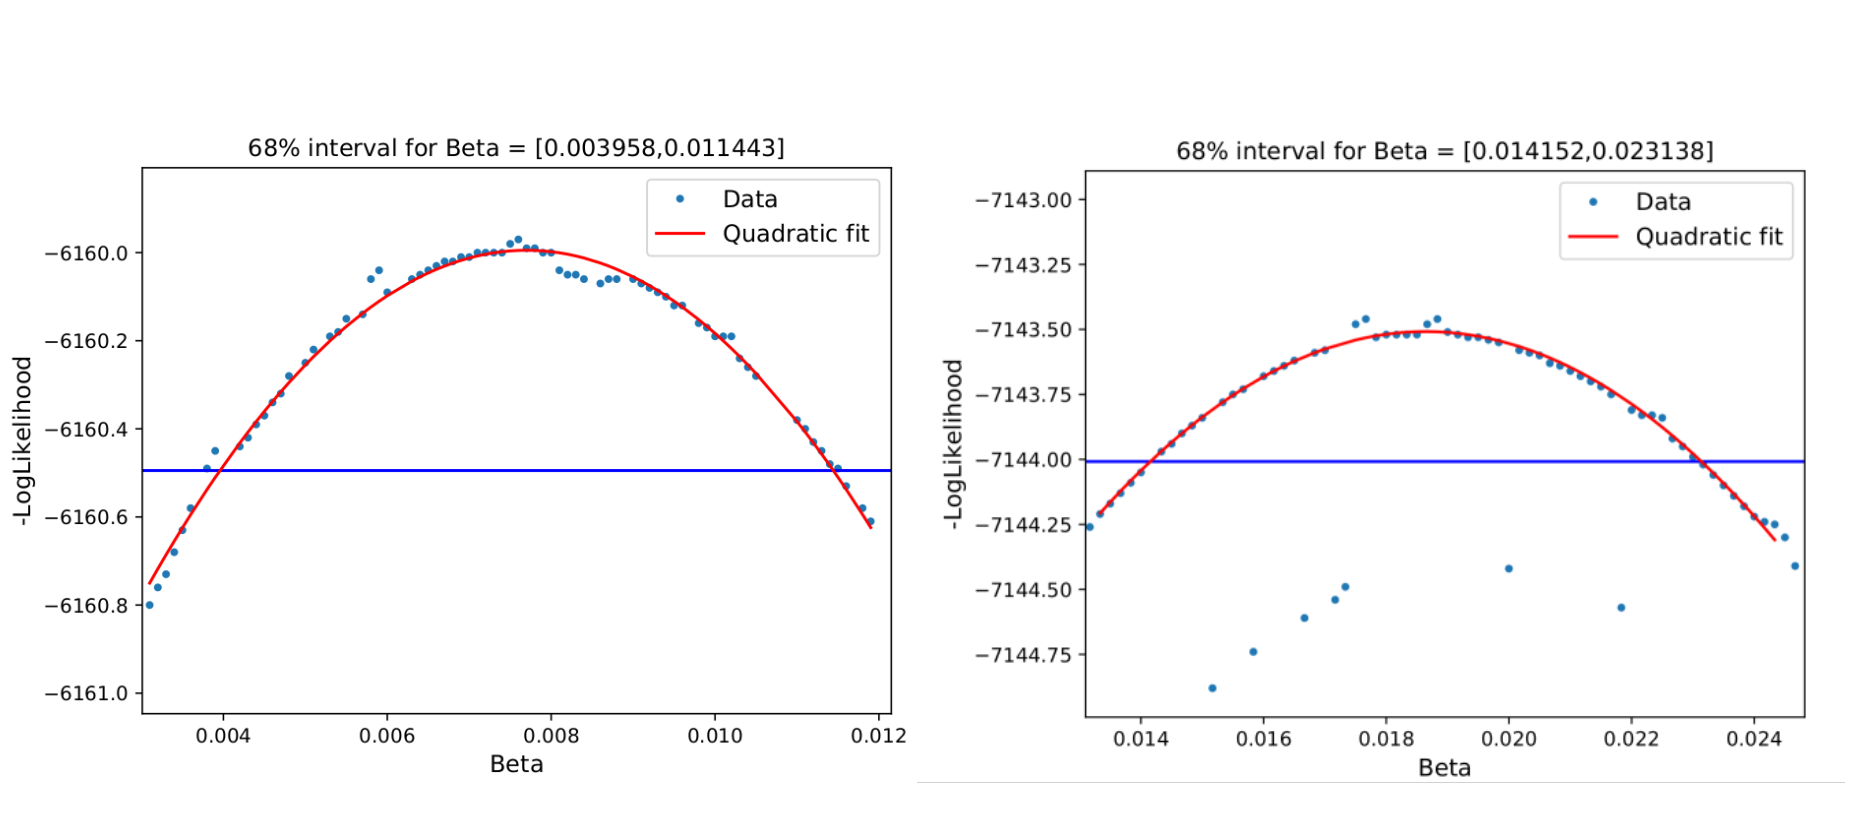
\includegraphics[scale=0.25]{pngs/Al_barridos_beta.png}
    \caption{\footnotesize{COMPLETAR.}}
    \label{fig:Al_barridos_beta}
\end{figure}
Los valores óptimos obtenidos de los ajustes se encuentran condensados en la Tabla \ref{tab:Al_FanoEehOHDU1y3}.
\ref{fig:Al_mu_sigma_fano}.
\begin{table}[h]
\centering
\begin{tabular}{@{}ccccc@{}}
\toprule
                & \multicolumn{2}{c}{OHDU1}                 & \multicolumn{2}{c}{OHDU3}                 \\ \hline\hline
                & $F$                 & $\varepsilon_{\eh}$ & $F$                 & $\varepsilon_{\eh}$ \\
EPIX 0.5 & $0.1322 \pm 0.0022$ & $3.7141 \pm 0.0019$ & $0.1498 \pm 0.0101$ & $3.7209 \pm 0.0029$ \\ 
EPIX 1.5 & $0.1455 \pm 0.0098$ & $3.7379 \pm 0.0024$ & $0.1699 \pm 0.0150$ & $3.7419 \pm 0.0039$ \\ 
EPIX 1.5 Corr & $0.1464 \pm 0.0096$ & $3.7501 \pm 0.0006$ & $0.1504 \pm 0.0011$ & $3.7485 \pm 0.0039$ \\ \bottomrule \hline
\end{tabular}
\caption{tabla}
\label{tab:Al_FanoEehOHDU1y3}
\end{table}
De esta se puede ver que por un lado se tiene que el valor del factor de Fano aumenta al pasar de \verb|EPIX=0.5| a \verb|EPIX=1.5|, al mismo tiempo que sus incertezas, tanto para el primer cuadrante como para el tercero, lo cual no era un resultado anticipable dado el aumento de estadística. El factor de Fano aumenta $\sim 10\,\%$ y su incerteza aumenta más de $4$ veces para el primer cuadrante, mientras que para el segundo el factor de Fano aumenta $\sim 12\,\%$y su incerteza un $\sim 50\,\%$.

Al aplicar las correcciones respecto al paso anterior lo que se obtiene es una ligera disminución del valor del Fano para el primer cuadrante, menor al $1\,\%$, y otra no tan ligera disminución para el tercero, cerda del $\sim 12\,\%$, donde curiosamente las incertezas no se comportan de la misma manera para ambos casos: Para el primer cuadrante la incerteza aumenta levemente, $\sim 3\,\%$, mientras que para el tercero disminuye muchísimo, mas del $\sim 95\,\%$. Todo esto puede verse con mayor claridad en el tercer gráfico de la Figura \ref{fig:Al_mu_sigma_fano}. Cabe destacar que los valores del factor de Fano para ambos cuadrantes se solapan con su error, de forma que los resultados para ambos cuadrantes resultan compatibles.

En los gráficos de la Figura \ref{fig:Al_OHDU1y3_EPIX15_Corr} se pueden ver los histogramas de carga del aluminio, obtenidos de los datos procesados con el umbral y las correcciones aplicadas con su ajuste, para los cuadrantes uno y tres, fijando el valor de $\beta$ en el máximo obtenido anteriormente para derivar el $F$ y $\varepsilon_{\eh}$ óptimos. En ambos gráficos se encuentran los histogramas de carga con el umbral \verb|EPIX=1.5| aplicado y superpuestos encima los histogramas de carga con el umbral \verb|EPIX=1.5| y las correcciones a la carga de los clusters. De esta forma se observa que las correcciones no modifican cualitativamente los histogramas.
\begin{figure}[h]
    \centering
        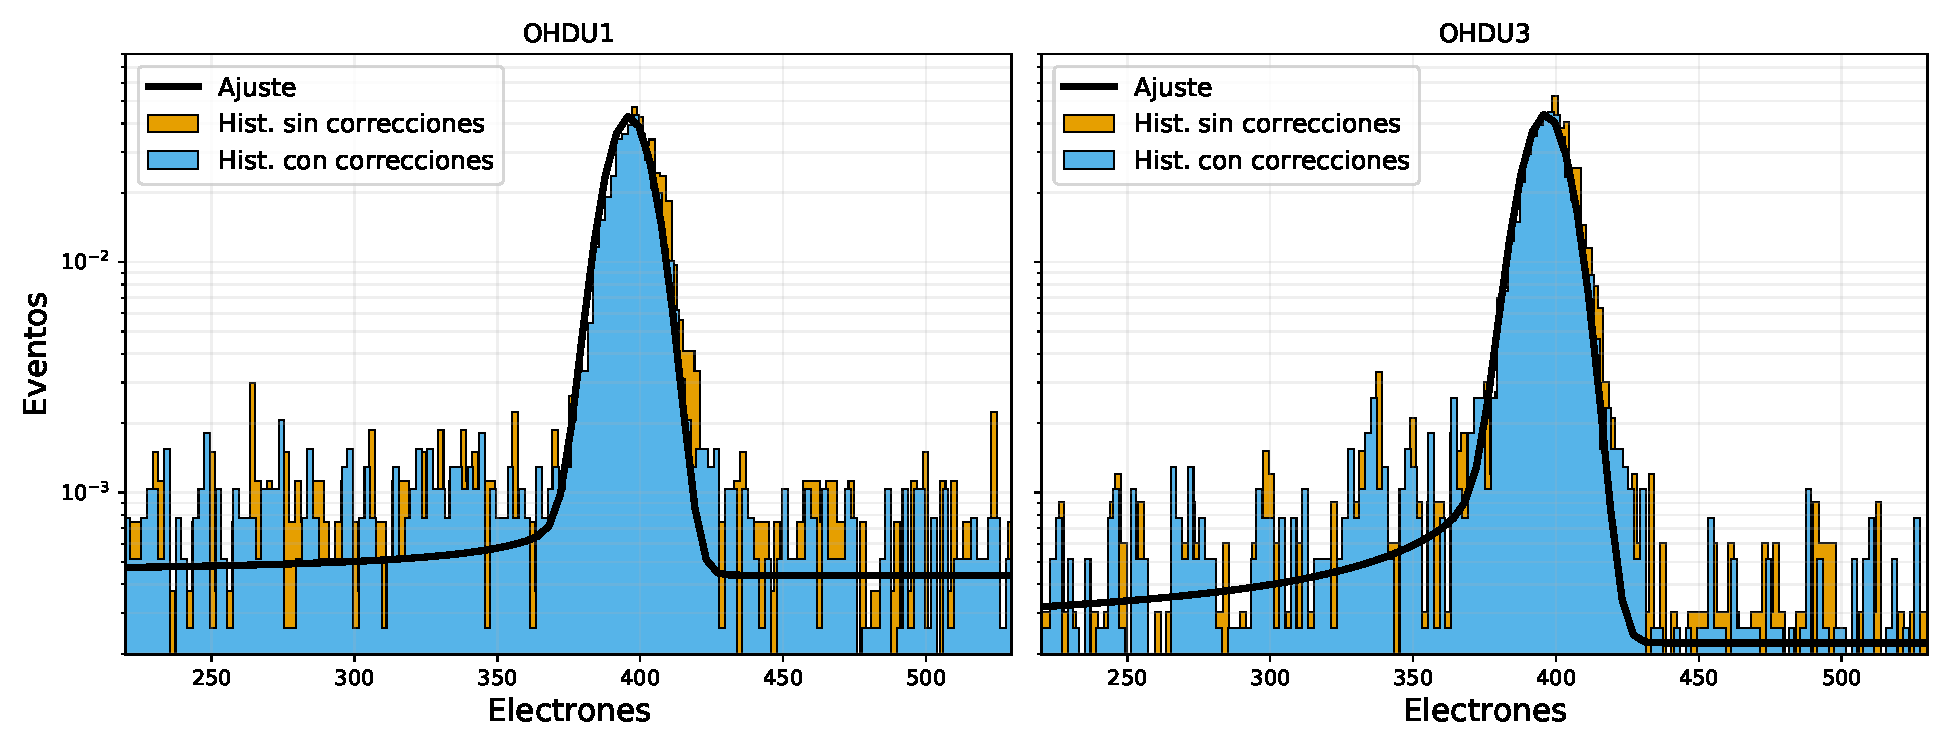
\includegraphics[scale=0.5]{Figs/Al_hists_ohdu1y3_dobles.pdf}
    \caption{\footnotesize{Histograma y ajuste del pico de los rayos $X$ del aluminio utilizando el modelo. El efecto de la colección parcial de carga es leve pero apreciable.}}
    \label{fig:Al_OHDU1y3_EPIX15_Corr}
\end{figure}

\begin{figure}[h]
    \centering
        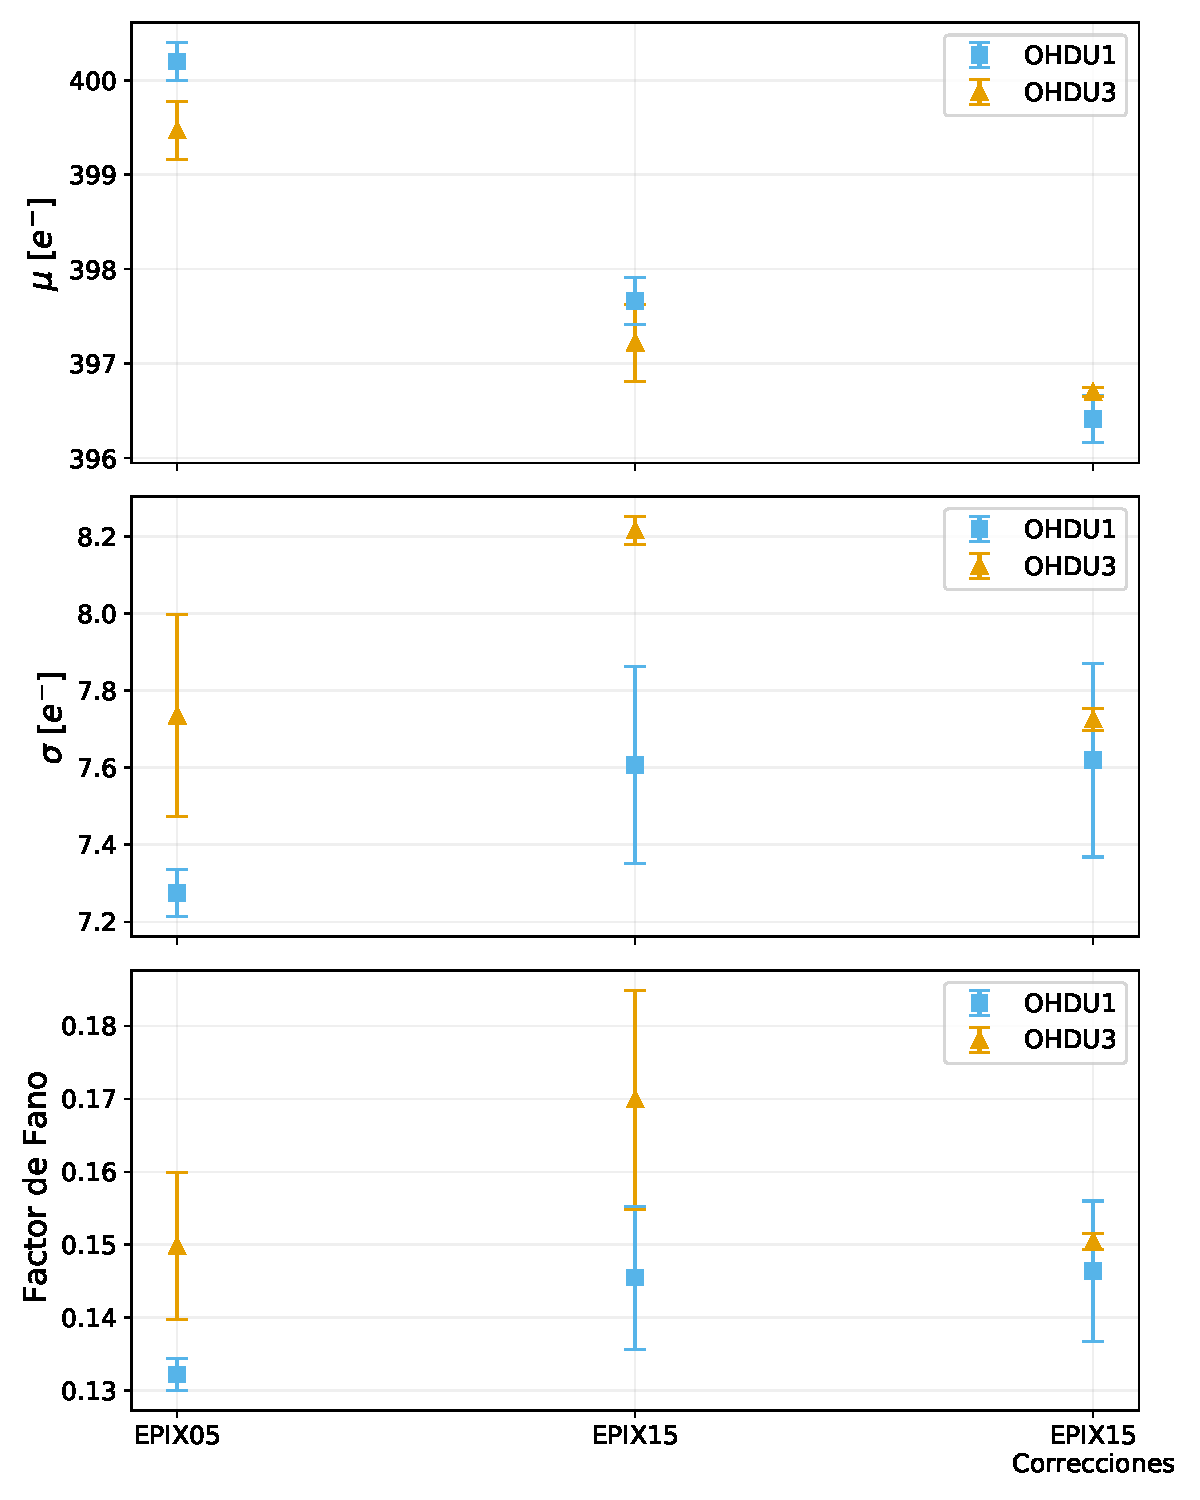
\includegraphics[scale=0.5]{Figs/Al_mu_sigma_fano.pdf}
    \caption{\footnotesize{Valores para las magnitudes relevantes para el factor de Fano, para los cuadrantes uno y tres, para los tres pasos de análisis implementados. Arriba: Valor medio del pico de rayos $X$ del aluminio; medio: Dispersión de los picos; abajo: factor de Fano. Se observa que la tendencia del factor de Fano sigue la misma tendencia de la dispersión.}}
    \label{fig:Al_mu_sigma_fano}
\end{figure}

Es interesante notar que el aumento del factor de Fano al aplicar el umbral se debe a un aumento de la dispersión de los picos, $\sigma$, como se ve en el segundo gráfico de la Figura \ref{fig:Al_mu_sigma_fano}. Es decir, al aumentar la estadística también aumenta el ancho de los picos.

En cuanto a la energía de creación electrón-hueco, para cada paso del análisis su valor aumentó, como puede verse en el gráfico de la Figura \ref{fig:Al_energia_creacion_eh}. En este caso el aumento de la estadística y las correcciones implementadas compatibilizaron los resultados entre los dos cuadrantes dado que sus incertezas se solapan y sus valores absolutos difieren menos de $0.1\,\%$.
\begin{figure}[h]
    \centering
        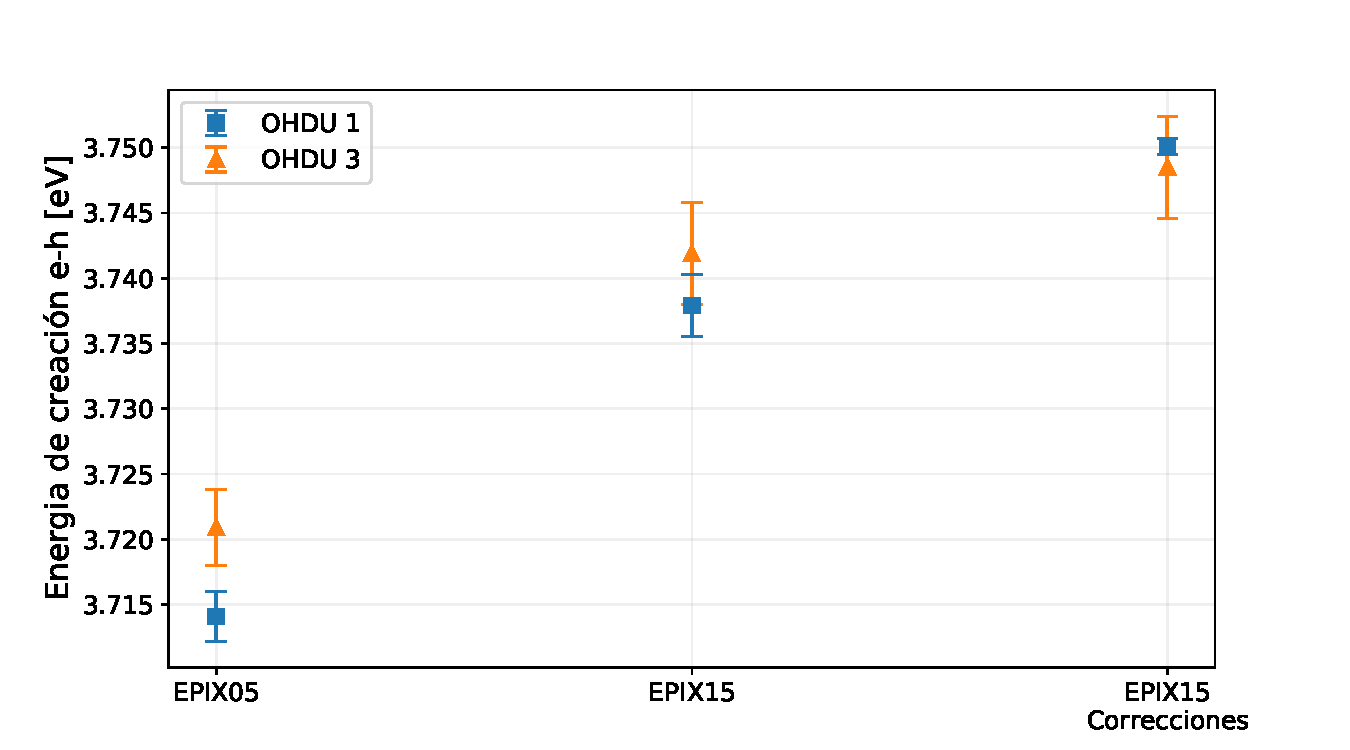
\includegraphics[scale=0.5]{Figs/Al_energia_creacion_eh.pdf}
    \caption{\footnotesize{asd.}}
    \label{fig:Al_energia_creacion_eh}
\end{figure}

%%%%%%%%%%%%%%%%%%%%%%%%%%%%%%%%%%%%%%%%%%%%%%%%%%%%%%%%%%%%%%%%%%
%%%%%%%%%%%%%%%%%%%%%%%%%%%%%%%%%%%%%%%%%%%%%%%%%%%%%%%%%%%%%%%%%%
\pagebreak
\subsection{Fluor}
\noindent Repitiendo el análisis realizado para el aluminio, se realizaron barridos en $\beta$ para obtener las curvas del logaritmo de la verosimilitud, de las cuales se obtienen el $\hat{\beta}$ máximo y los extremos de los intervalos para cada cuadrante, como se ve en la Figura \ref{fig:F_barridos_beta}.%
En este caso se ve que la curva obtenida para el tercer cuadrante no se aproxima por una cuadrática y no fue ajustada, con lo cual usar $\ln{(L(\hat{\beta}))} - 1/2$ para establecer el intervalo de $68.3\,\%$ no es correcto.%
Sin embargo para el primer cuadrante el ajuste cuadrático está en muy buen acuerdo con los valores obtenidos y de estos se desprende $\hat{\beta} = 0.232$, con su intervalo $[0.2193; 0.2450]$ de $68.3\,\%$.

En este caso, sabiendo que la longitud de atenuación en el silicio para los rayos $X$ del flúor de $677\,\si{eV}$ es de $\tau_{\scaleto{X}{4pt}} = 0.941\,\si{\mu m}$\cite{AttenuationLength}, se obtiene que el ancho de la región de PCC del detector es de $\tau_{\scaleto{CCE}{4pt}} = 0.218\,\si{\mu m}$, contenido en el intervalo $[0.2063; 0.2306]\,\si{\mu m}$.
\begin{figure}[h]
    \centering
    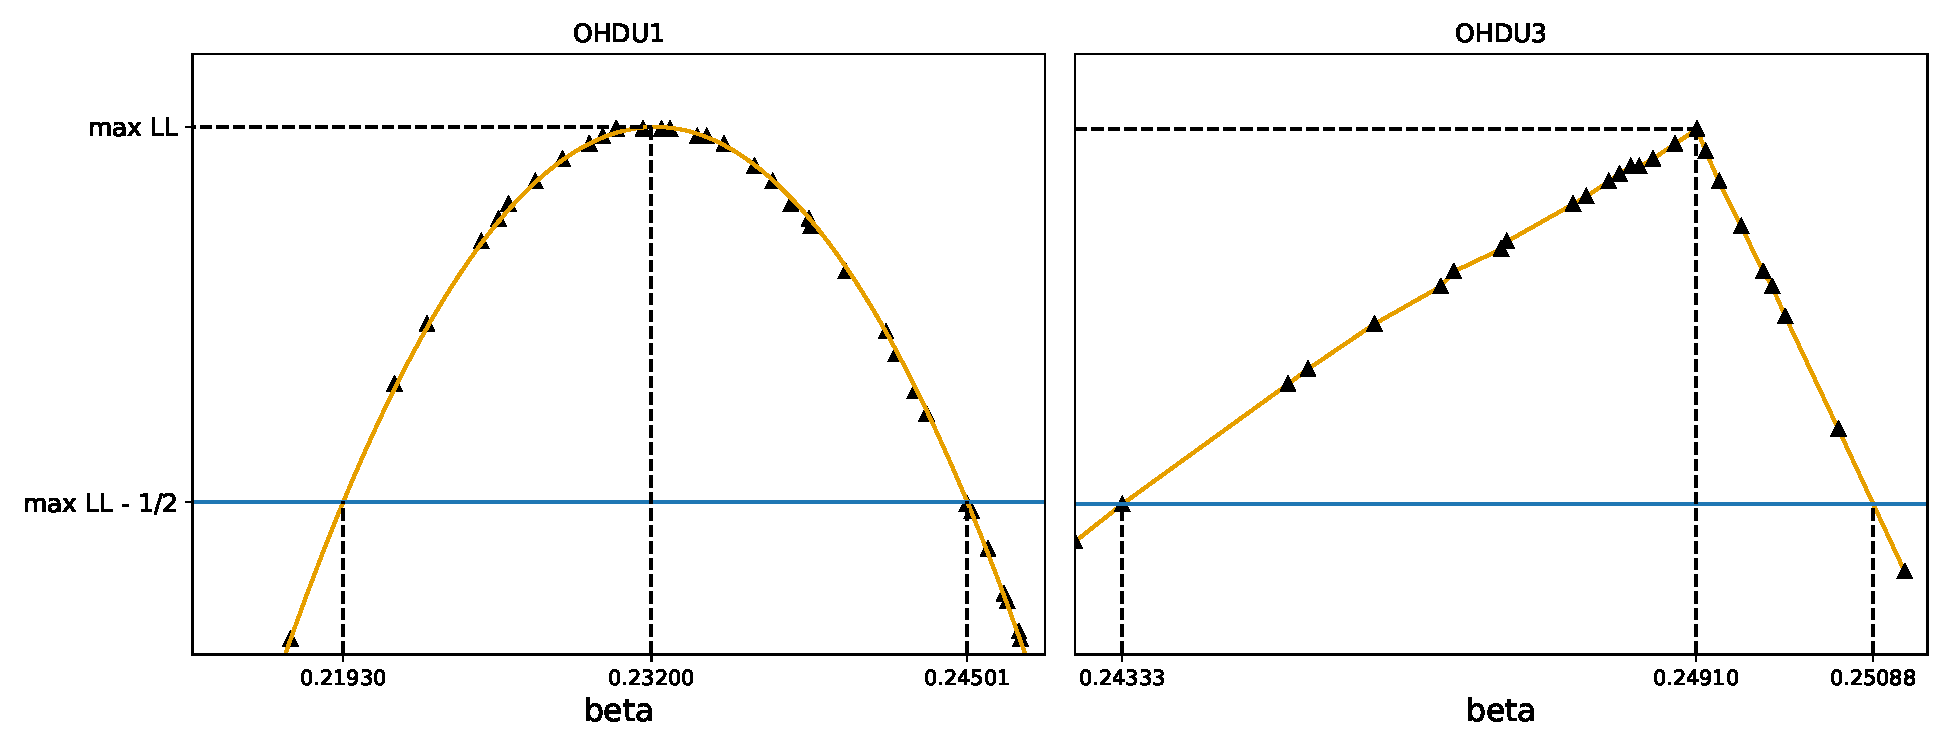
\includegraphics[scale=0.5]{Figs/F_barridos_beta.pdf}
    \caption{\footnotesize{\textbf{completar}}}
    \label{fig:F_barridos_beta}
\end{figure}
Con el valor $\hat{\beta}$ hallado para el primer cuadrante, se realizaron los ajustes a los histogramas de carga ambos cuadrantes y se obtuvieron los valores para el factor de Fano y energía de creación electrón-hueco. De la misma forma que para el aluminio, en la Figura \ref{fig:F_OHDU1y3_EPIX15conCorr} se tienen los histogramas de carga con y sin corrección, y con su respectivo ajuste. Se observa como la colección parcial de carga afecta a estos picos de forma mucho más pronunciada que para el aluminio, formando colas muy pronunciadas a la izquierdo de estos. Esto es un resultado que se anticipaba en el Capítulo \ref{chap:ModeloPCC} y se debe al aumento del valor del parámetro $\beta$: como la longitud de atenuación para los rayos $X$ del flúor es mucho menor que la del aluminio, hay muchísimos más eventos que sufren recombinación en la región de PPC del sensor. 
\begin{figure}[h]
    \centering
    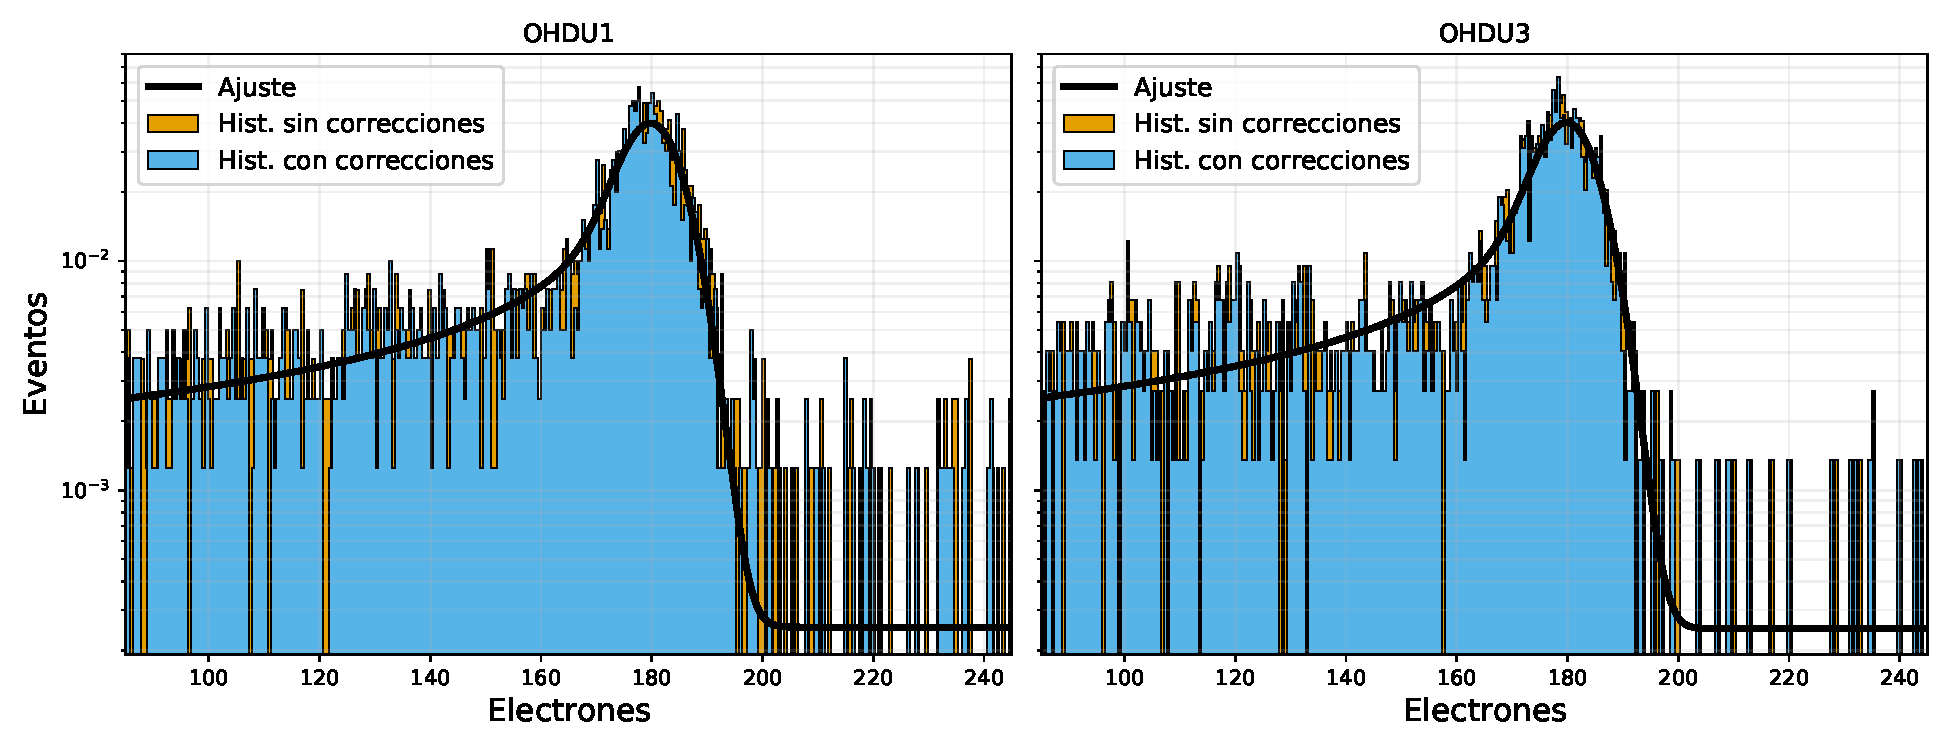
\includegraphics[scale=0.5]{Figs/F_hists_ohdu1y3_dobles.pdf}
    \caption{\footnotesize{\textbf{completar}}}
    \label{fig:F_OHDU1y3_EPIX15conCorr}
\end{figure}
En la Tabla \ref{tab:F_FanoEehOHDU1y3} se presentan los resultados para los tres pasos del análisis para los cuadrantes uno y tres.
\begin{table}[h]
\centering
\begin{tabular}{@{}ccccc@{}}
\toprule
                & \multicolumn{2}{c}{OHDU1}                 & \multicolumn{2}{c}{OHDU3}                 \\ \hline\hline
                & $F$                 & $\varepsilon_{\eh}$ & $F$                 & $\varepsilon_{\eh}$ \\
EPIX 0.5 & $0.1225 \pm 0.0112 $ & $3.6576 \pm 0.0006 $ & $0.1304 \pm 0.0106 $ & $3.6778 \pm 0.0050 $ \\ 
EPIX 1.5 & $0.1415 \pm 0.0202 $ & $3.7363 \pm 0.0097 $ & $0.1416 \pm 0.0120 $ & $3.7363 \pm 0.0065 $ \\ 
EPIX 1.5 Corr & $0.1415 \pm 0.0170 $ & $3.7363 \pm 0.0066 $ & $0.1417 \pm 0.0169 $ & $3.7363 \pm 0.0066$ \\ \bottomrule \hline
\end{tabular}
\caption{tabla}
\label{tab:F_FanoEehOHDU1y3}
\end{table}

En los gráficos de la Figura \ref{fig:F_mu_sigma_fano} se ven estas tendencias con sus errores. En todos los casos los errores de las magnitudes se solapan al aplicar las correcciones. También se ve que nuevamente la tendencia del factor de Fano se rige por la tendencia de la dispersión $\sigma$ del pico.
\begin{figure}[h]
    \centering
        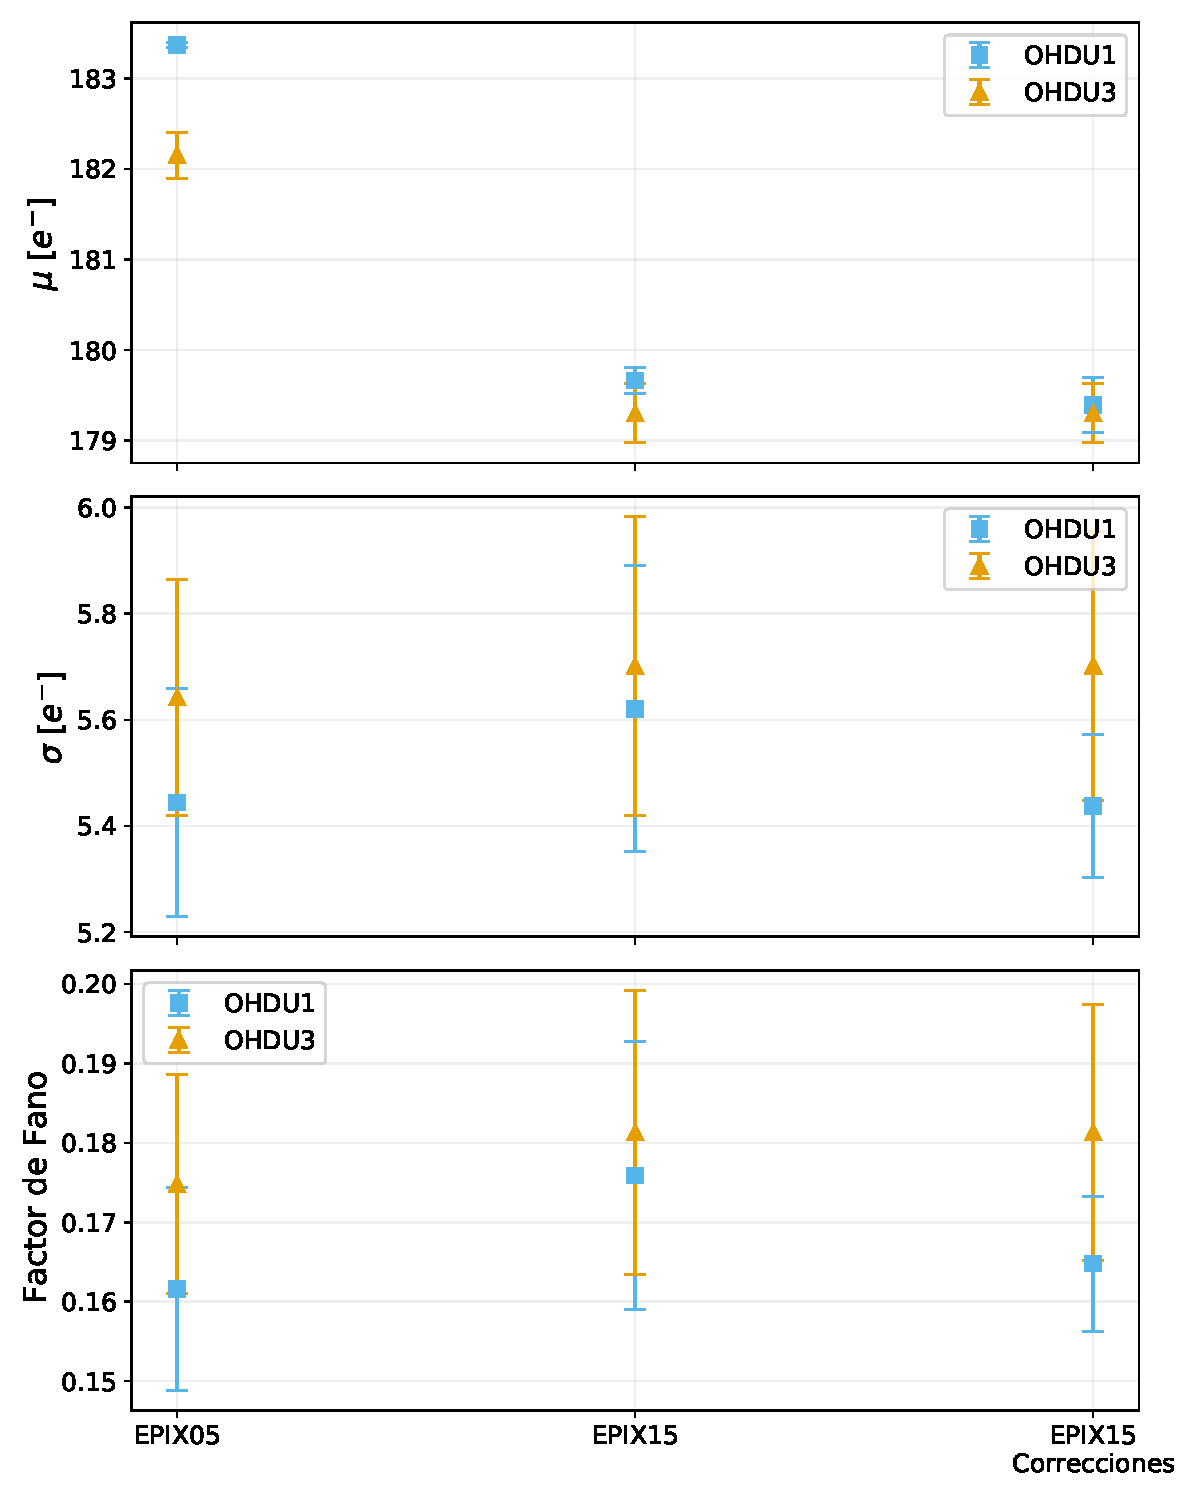
\includegraphics[scale=0.5]{Figs/F_mu_sigma_fano.pdf}
    \caption{\footnotesize{asd.}}
    \label{fig:F_mu_sigma_fano}
\end{figure}

La energía de creación electrón-hueco, por su parte, aumentó al aplicar el umbral y luego de aplicar las correcciones se mantuvieron los valores y se solaparon los errores entre los cuadrantes.
\begin{figure}[h]
    \centering
        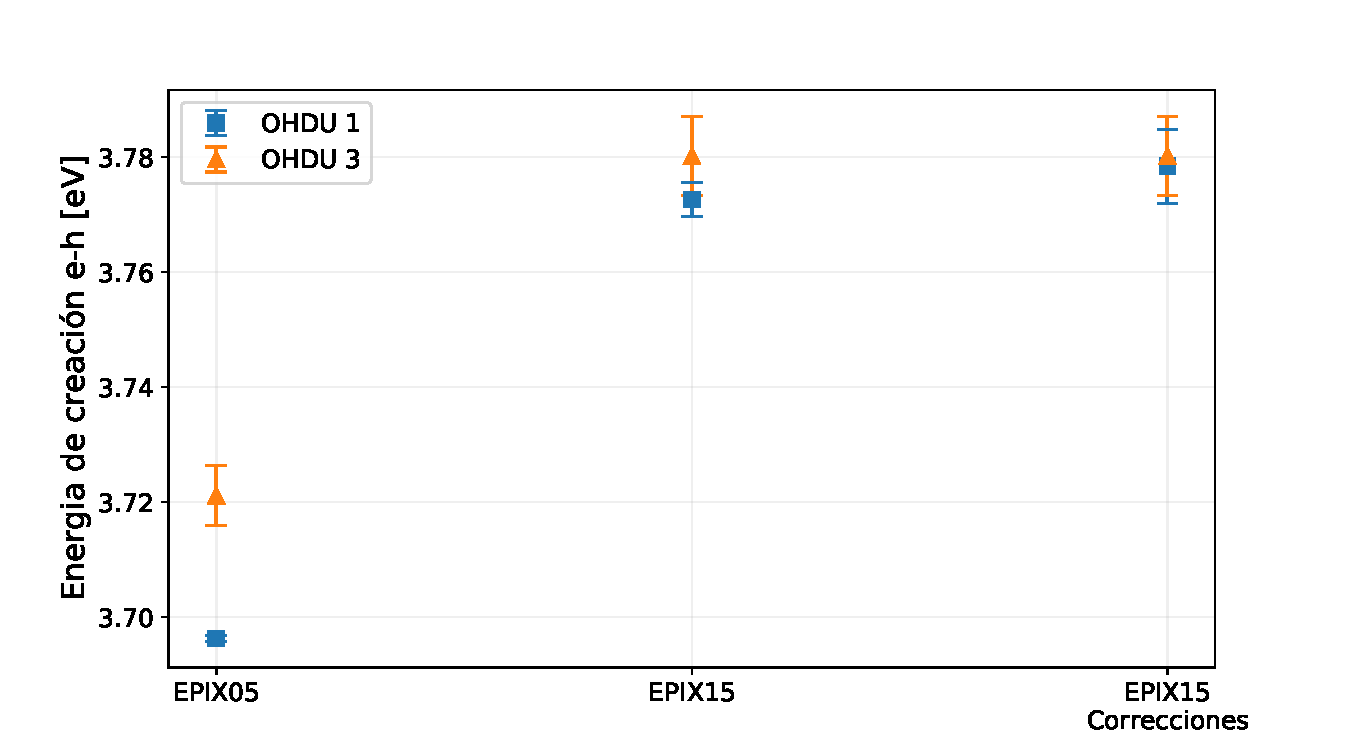
\includegraphics[scale=0.5]{Figs/F_energia_creacion_eh.pdf}
    \caption{\footnotesize{asd.}}
    \label{fig:F_energia_creacion_eh}
\end{figure}
Finalmente, no se obtuvieron mejoras apreciables en las incertezas de las magnitudes a pesar del aumento de la estadística provocado por el nuevo umbral utilizado. Sin embargo, el procedimiento utilizado para la corrección de los sesgos logra compatibilizar los cuadrantes uno y tres tanto para el factor de Fano como para el energía de creación electrón-hueco, para los rayos $X$ del aluminio y del flúor. Por otro lado, estos resultados también ponen de manifiesto la ventaja de la utilización de este nuevo modelo de ajuste, debido a que a partir de este tipo de mediciones se puede obtener el ancho de la región de colección parcial de carga del detector.
